\section{Force Test Journal} \label{forceTestJournal} %<-- remember to label your test so you can
%\textbf{Name: Group 630}\\  %    reference in the appropriate section
\textbf{Date: Aug. 10, 2018}

\subsubsection{Purpose}
The purpose of the test is to measure the force on the cart directly in relation to the input given by the microcontroller to ensure that the relation between the 12 bit input and the actual force output is accurate.

\subsubsection{Setup}
\begin{figure}[H]
	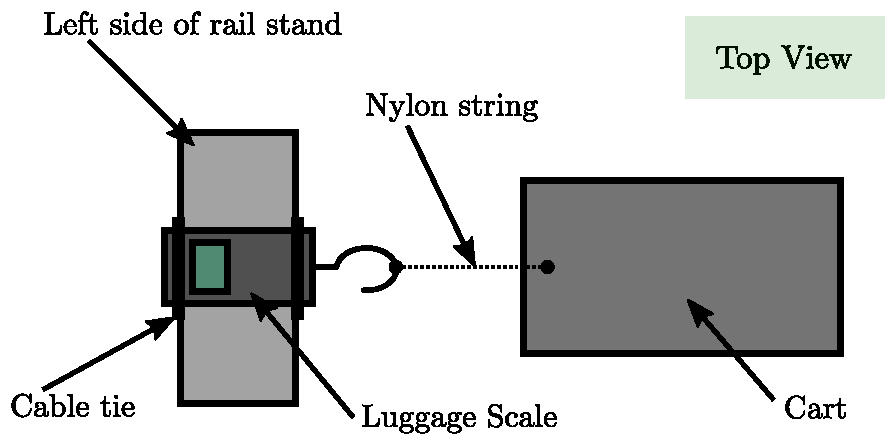
\includegraphics[scale=.45]{figures/testSetup}
	\caption{Setup diagram}
  \label{testSetup}
\end{figure}

\subsubsection{List of Equipment}
\begin{table}[H]
\begin{tabular}{|l|l|}
\hline%------------------------------------------------------------------------------------
  \textbf{Instrument}                        &   \textbf{Type}                           \\
\hline%------------------------------------------------------------------------------------
  Cart pendulum                              &   Setup at AAU Control Lab                \\
\hline%------------------------------------------------------------------------------------
   Laptop             	     	               &   Asus UX31E                              \\
\hline%------------------------------------------------------------------------------------
   Luggage scale                             &   B00ZWNGZFO ES-PS01                      \\
\hline%------------------------------------------------------------------------------------
  Cable ties for mounting the Luggage scale  &                                           \\
\hline%------------------------------------------------------------------------------------
   Nylon string for attaching the scale to the cart  &                                   \\
\hline%------------------------------------------------------------------------------------
\end{tabular}
\end{table}

\subsubsection{Procedure}

\begin{enumerate}
  \item Attach the luggage scale to the setup using the cable ties as seen in \autoref{testSetup}.
  \item Attach the cart to the luggage scale as seen in \autoref{testSetup}.
  \item Power up the setup.
  \item Connect the Teensy in the setup through USB to the laptop.
  \item Ready and compile the code giving a constant reference\\ of \SI{1.3}{A} (supposed) armature current.
  \item Upload the code to the Teensy board.
  \item Take reading of the the weight pulled by the cart.
  \item repeat step 5 to 7 with \SI{0.1}{A} increments\\ for each measurement up to \SI{4.5}{A}.
\end{enumerate}

\subsubsection{Results}

\begin{table}[H]
\flushleft
\begin{tabular}{|l|l|l| l|l|l| l|l|l| l|l|}
\cline{1-2}\cline{4-5}\cline{7-8}\cline{10-11}%----------  ----------------------------  ----------------------------
  \textbf{[A]} & \textbf{[kg]} &\phantom{h}& \textbf{[A]} & \textbf{[kg]}  &\phantom{h}& \textbf{[A]} & \textbf{[kg]} &\phantom{h}& \textbf{[A]} & \textbf{[kg]} \\
\cline{1-2}\cline{4-5}\cline{7-8}\cline{10-11}%----------  ----------------------------  ----------------------------
  \num{1.3} & \num{0.30}   &   & \num{2.1} & \num{0.66} &  & \num{2.9}  & \num{0.86}  &  & \num{3.7}  & \num{1.11} \\
\cline{1-2}\cline{4-5}\cline{7-8}\cline{10-11}%----------  ----------------------------  ----------------------------
  \num{1.4} & \num{0.36}   &   & \num{2.2} & \num{0.71} &  & \num{3.0}  & \num{0.90}  &  & \num{3.8}  & \num{1.16} \\
\cline{1-2}\cline{4-5}\cline{7-8}\cline{10-11}%----------  ----------------------------  ----------------------------
  \num{1.5} & \num{0.40}   &   & \num{2.3} & \num{0.73} &  & \num{3.1}  & \num{0.92}  &  & \num{3.9}  & \num{1.17} \\
\cline{1-2}\cline{4-5}\cline{7-8}\cline{10-11}%----------  ----------------------------  ----------------------------
  \num{1.6} & \num{0.46}   &   & \num{2.4} & \num{0.75} &  & \num{3.2}  & \num{0.95}  &  & \num{4.0}  & \num{1.20} \\
\cline{1-2}\cline{4-5}\cline{7-8}\cline{10-11}%----------  ----------------------------  ----------------------------
  \num{1.7} & \num{0.47}   &   & \num{2.5} & \num{0.78} &  & \num{3.3}  & \num{0.97}  &  & \num{4.1}  & \num{1.22} \\
\cline{1-2}\cline{4-5}\cline{7-8}\cline{10-11}%----------  ----------------------------  ----------------------------
  \num{1.8} & \num{0.53}   &   & \num{2.6} & \num{0.80} &  & \num{3.4}  & \num{1.02}  &  & \num{4.2}  & \num{1.26} \\
\cline{1-2}\cline{4-5}\cline{7-8}\cline{10-11}%----------  ----------------------------  ----------------------------
  \num{1.9} & \num{0.55}   &   & \num{2.7} & \num{0.82} &  & \num{3.5}  & \num{1.05}  &  & \num{4.3}  & \num{1.28} \\
\cline{1-2}\cline{4-5}\cline{7-8}\cline{10-11}%----------  ----------------------------  ----------------------------
  \num{2.0} & \num{0.63}   &   & \num{2.8} & \num{0.84} &  & \num{3.6}  & \num{1.08}  &  & \num{4.4}  & \num{1.32} \\
\cline{1-2}\cline{4-5}\cline{7-8}\cline{10-11}%----------  ----------------------------  ----------------------------
   \multicolumn{9}{l|}{}                                                                 & \num{4.5}  & \num{1.34} \\
\cline{10-11}%                                                                           ----------------------------
\end{tabular}
\end{table}
%
To obtain the forces, $F$ [\si{N}], all readings, [\si{kg}], are multiplied by the gravitational acceleration $g=$\nolinebreak\ \SI{9.82}{m\cdot s^{-1}}.
\pagebreak